
\documentclass[%
 %reprint,
%superscriptaddress,
%groupedaddress,
%unsortedaddress,
%runinaddress,
%frontmatterverbose, 
preprint,
%preprintnumbers,
%nofootinbib,
%nobibnotes,
%bibnotes,
 amsmath,amssymb,
 aps,
%pra,
%prb,
%rmp,
%prstab,
%prstper,
%floatfix,
]{revtex4}


\usepackage{aas_macros}
\usepackage{amssymb}
\usepackage{amsmath}
\usepackage{array}
\usepackage{graphicx}
\usepackage{color,units}
\usepackage[dvipsnames]{xcolor} % for more colours!

\usepackage{lineno}
\usepackage{xspace}
\usepackage{dcolumn}
\usepackage{longtable}
\usepackage[normalem]{ulem} %% for striking out text
\usepackage{subfigure}
\usepackage[T1]{fontenc}
\usepackage{hyperref}


\usepackage{dcolumn}% Align table columns on decimal point
\usepackage{booktabs}
\usepackage{xspace} 
\usepackage{bm}% bold math
\usepackage{hyperref}% add hypertext capabilities
\usepackage{graphicx} % Include figure files
\graphicspath{{Figures/}} %Setting the graphicspath

                 % Astronomical Journal

\newcommand{\prior}{{\sc prior}\xspace}
\newcommand{\bilby}{{\sc \href{https://lscsoft.docs.ligo.org/bilby/}{\texttt{Bilby}}}\xspace}
\newcommand{\bilbypipe}{{\sc bilby\_pipe}\xspace}
\newcommand{\pbilby}{{\sc pBilby}\xspace}
\newcommand{\dynesty}{{\sc dynesty}\xspace}
\newcommand{\cpnest}{{\sc cpnest}\xspace}
\newcommand{\ptemcee}{{\sc ptemcee}\xspace}
\newcommand{\gwpy}{{\sc \href{https://gwpy.github.io/}{\texttt{GWpy}}}\xspace}
\newcommand{\imrphenomp}{{\sc IMRPhenomPv2}\xspace}
\newcommand{\seob}{{\sc SEOBNRv4PHM}\xspace}
\newcommand{\pycbc}{{\sc \href{https://pycbc.org/}{\texttt{PyCBC}}}\xspace}
\newcommand{\bcr}{{\sc BCR}\xspace}
\newcommand{\psd}{{\sc $\sigma^2_i$}\xspace}
\newcommand{\pastro}{{\sc $p_\text{astro}$}\xspace}
\newcommand{\msun}{{\sc M${}_\odot$}\xspace}
\newcommand{\template}{{\sc $\mu(\vec{\theta})$}\xspace}
\newcommand{\parameters}{{\sc $\vec{\theta}$}\xspace}


\newcommand{\av}[1]{\textcolor{orange}{[AV: #1]}}
\newcommand{\rs}[1]{\textcolor{red}{[RS: #1]}}
\newcommand{\et}[1]{\textcolor{blue}{[ET: #1]}}


\begin{document}

\preprint{APS/123-QED}

\title{A Bayesian search to find \\high-mass black holes in LIGO data}% Force line breaks with \\



\author{Author list TBD}

\date{\today}

\begin{abstract}

The detection of high mass black holes ( $>100$ \msun) will shed light on the formation of supermassive black holes and thus galaxy formation. Although LIGO is sensitive to the merger of binary black holes with total masses up to 500 \msun, the largest total mass detected so far is approximately $80$ \msun. A possible explanation for the absence of high mass events may be due to their misclassification as short-duration instrumental noise transients. Short-duration instrumental transients mimic the short-duration gravitational-wave signals from high-mass binary black hole mergers. Here we demonstrate that a new search method utilising Bayesian inference could be a more sensitive tool for detecting high-mass binary black hole mergers as compared to traditional match-filtering. We have applied this technique on the high-mass triggers during LIGO's second observing run to investigate the possibility of discovering new gravitational-wave signals from an entirely new class of high mass black hole binaries. \rs{add sentence describing if we see any new events; add a sentence on our analysis of IAS events}



\end{abstract}

\maketitle

%\tableofcontents


%%%%%%---SECTIONS---%%%%%%%%%%%%
\section{\label{sec:Introduction}Introduction}
\av{Need to edit in light of S190521G paper}
Since the 1970s, there has been an accumulation of evidence for stellar-mass and supermassive black holes. In 2019, the Event Horizon Telescope provided the first visual evidence of the supermassive black hole M87  \cite{m87photo}.  As of January 2020, LIGO, Virgo and IAS \rs{we should think carefully about how to describe the IAS events here; I think our conclusion is that they're not real} have confirmed more than a dozen binary black hole systems \cite{GWTC1, IAS0, IAS1, IAS2, pycbc_ogc_2}. These various discoveries have firmly established the existence of stellar-mass black holes, supermassive black holes and binary black hole systems.  Interestingly, there is still no direct evidence for intermediate-mass black holes, the black holes that lie in between stellar-mass and supermassive black hole systems with masses between $10^2-10^6$ \msun. Thus, the existence of intermediate-mass black holes is still speculative. \\

If intermediate-mass black holes are present, the gravitational waves emitted from the merger of a binary black hole system with at least one intermediate-mass black hole (up to a mass of $400$ \msun) will be detectable by the ground-based gravitational-wave network. Gravitational waves from such systems should occur at a rate of $0-10\text{yr}^{-1}$ \cite{fregeau2006imbhbRatePrediction, mandel2008rates,rodriguez2015bbhRatePredictions}.  However, even after conducting a targeted matched-filter based search for gravitational waves from intermediate-mass black holes the largest total mass detected so far is approximately $80$ \msun \cite{imbhbSearch2014, ligo_imbh_search, abbott2019gwtc}. A possible explanation for the absence of intermediate-mass events may be due to their misclassification as short-duration instrumental noise transients known as glitches \cite{glitch_in_fifth_ligo_run, bayeswave, improving_dq_in_early_runs, ligo_glitch_gw150914, pycbc_short_duration_transients, pe_with_glitch, blip_glitches}. These glitches can mimic astrophysical signals and hence decrease the significance of true gravitational wave events. \\

One method to account for glitches while searching for gravitational waves from coalescing compact binaries is by utilising an astrophysical Bayesian odds  \cite{bci, BCR1, BCR2, bcr_gw151216, bayesian_odds}. A true Bayesian odds calculated without using bootstrap techniques can provide events with a more accurate significance that is agnostic to a specific search strategy \cite{BCR2, bcr_gw151216,  bayesian_odds}. Additionally, a Bayesian odds can include more information than is included in current matched filter searches such as if the gravitational wave event's signal is coherent amongst the network of detectors, if the binary system that created the gravitational waves was precessing, and if the gravitational wave signal contains higher-order modes.  It is because Bayesian methods can incorporate all this physical information about a gravitational wave signal that the LIGO Scientific Collaboration uses these methods to determine the source parameters of gravitational wave events \cite{abbott2016ligo, abbott2019gwtc}. This paper demonstrates that the power of Bayesian methods used in parameter estimation can also successfully be used to discriminate between coherent gravitational-wave signals, incoherent glitches, and Gaussian noise in the form of a Bayesian search. \\

In this paper we utilise a Bayesian method, called the \bcr \cite{BCR1}, to search for the significant gravitational wave signals from high-mass (systems with total masses in the range of $55-500$ \msun) compact binary coalescences in the detector data recorded during aLIGO's second observing run (O2).  We find that (a) our search does not identify any unreported stellar mass or intermediate mass black holes; (b) high-mass events reported in the GWTC-1, including GW170729 (an event with disputed $p_\text{astro}$ amongst various search pipelines) have high low significance; and that (c) high-mass events detected from some independent groups have low significance. \rs{explicitly state that they're the IAS events}\\

The remainder of this paper is structured as follows. We outline our methods, including details of the \bcr and the retrieval of our candidate events in Section~\ref{sec:method}. We present details on the implementation of our analysis in Section~\ref{sec:Analysis}. Finally we present our results in Section~\ref{sec:Results}, and discuss these results in the context of the significance of gravitational wave candidates in Section~\ref{sec:Conclusion}.


\section{Method\label{sec:method}}
\rs{I think you need a synopsis of this section before going into the details; explain that one could in principle apply bayesian methods only, but we don't do that here. Instead, we take triggers from pycbc and use bayesian evidences as a ranking statistic etc...} 
\subsection{Triggers for Analysis}
The LIGO Scientific collaboration runs a number of search pipelines that target gravitational waves from compact binary mergers such as the GstLAL, MBTA, SPIIR and PyCBC searches \cite{abbott2019gwtc}.\\

At its core, the \pycbc \cite{pycbc_code} search performs a matched-filter search for binary merger signals by comparing the data against templates from a gravitational-wave template-bank \cite{pycbc_og6}. \sout{\pycbc calculates the matched-filter for several different coalescence times and uses numerous templates from the template bank for each section of data being analysed.} The output of \pycbc's search is a signal-to-noise ratio $\rho$ like statistic, called the \pycbc ranking statistic $\rho_\text{PC}$. This statistic is a function of the matched-filter $\rho$, signal-based veto values, intrinsic and extrinsic properties of the apparent signal and other information \cite{pycbc_og6}. Whenever a local maximum of $\rho_\text{PC} > \rho_\text{T}$, where $\rho_\text{T}$ is some threshold value, the search pipeline produces a single-detector trigger associated with the detector and time where the data was obtained.\\

For \pycbc to consider a trigger to be a \textbf{candidate trigger}, a trigger from astrophysical origins, the trigger must be observed between detectors with the same template and a time of arrival difference less than the gravitational-wave travel time between detectors \cite{pycbc_og6}. To test its search, \pycbc also conducts searches for \textbf{simulated triggers}, artificial triggers manufactured by injecting signals into the detector data. These simulated signal studies provides \pycbc with metrics on its search's sensitivity. Finally, to quantify the statistical significance of candidate events, \pycbc artificially constructs a \textbf{background trigger} set to compare the candidate events against. These background triggers are signal-free events \rs{not quite: they contain signals, just not coherent ones}, constructed by applying relative offsets, or time-shifts, between the data of different detectors \cite{pycbc_og6}. Note that the time-shifts to generate the background triggers are greater than the gravitational-wave travel time between detectors to ensure that the background triggers are not of astrophysical origins. \\

In our work, we demonstrate that the \bcr can be used in a similar way as $\rho_\text{PC}$, as a ranking statistic, to measure the statistical significance of candidate triggers. Before we discuss how we use the \bcr as a measure of significance, we introduce the method to calculate the \bcr in the following section.\\


\subsection{The Bayesian Coherence Ratio}

Bayes theorem states that the probability $P(\mathcal{H}|d)$ for a hypothesis $\mathcal{H}$ and data $d$ is
\begin{equation}
    P(\mathcal{H}|d) = \frac{\mathcal{L}(d|\mathcal{H})\pi(\mathcal{H})}{Z}\ , 
\end{equation}
\rs{see comments from last week on replacing L wiht Z etc...}
where $\mathcal{L}(d|\mathcal{H})$ is the likelihood of the data given
the hypothesis,  $\pi(\mathcal{H})$ is the prior probability of the hypothesis, and finally, $Z = \sum \mathcal{L}(d|\mathcal{H})  \pi(\mathcal{H})$ is the marginalised likelihood called the evidence \av{Rory suggested we use $Z(d|H)$ instead of $L(D|H)$}.  To compare two hypotheses $\mathcal{H}_A$ and $\mathcal{H}_B$ with the Bayes theorem one can calculate an odds ratio
\begin{equation}
    \mathcal{O}^A_B = \frac{Z^A\ \pi(\mathcal{H}_A)}{Z^B\ \pi(\mathcal{H}_B)}\ ,
\end{equation}
where $Z^A$ and $Z^B$ are the evidences for the $\mathcal{H}_A$ and $\mathcal{H}_B$ hypotheses. The odds ratio can tell us which of the two hypotheses is more likely. For example, if $\mathcal{O}^A_B >> 1$, then this odds ratio indicates that the $\mathcal{H}_A$ is much more likely than $\mathcal{H}_B$. \\

The \bcr is a Bayesian odds ratio like the above, of a coherent signal hypotheses $\mathcal{H}_S$ and an incoherent instrumental feature hypothesis $\mathcal{H}_I$ for a network of $D$ detectors. $\mathcal{H_I}$ states that each detector $i$ has either pure Gaussian noise $\mathcal{H}_N$ or a glitch $\mathcal{H}_G$. Following \citet{BCR1}, the \bcr is given by
\begin{equation}
\label{eq:bcr}
\text{BCR} = \frac{\alpha Z^S}{\prod\limits^D_{i=1} \ [\beta Z^G_i + (1-\beta)Z^N_i]}\ ,
\end{equation}
where $Z^S$, $Z^G_i$ and $Z^N_i$ are the Bayesian evidences (marginalised likelihoods) for $\mathcal{H}_S$, $\mathcal{H}_N$, and $\mathcal{H}_G$. $\alpha$ and $\beta$, are the prior odds for obtaining a signal $\alpha=P(\mathcal{H}_S)/P(\mathcal{H}_I)$ and the prior odds for obtaining a glitch $\beta=P(\mathcal{H}_G)/P(\mathcal{H}_I)$. As the rate of signal and glitches are unknown, these priors $\alpha$ and $\beta$ are tuned to maximise the \bcr distributions for background data (signal-free data) and simulated signals \cite{BCR1}.  \\

\subsection{Bayesian Evidence Evaluation}
\subsubsection{Noise Model}
We assume that each detector's noise is Gaussian and stationary over the period being analysed \cite{ligo_psd}. In practice, we estimate the noise variance using the noise power spectral density (PSD)  \psd of the data. \rs{NOTE: $\sigma_i^2$ is the noise variance, not the PSD. If you compare the likelihood in, e.g., veitch and vecchio to yours you can see how to relate the variance to the PSD and vice versa}. Using the \psd, for each data segment $d_i$ in each of the $i$ detectors in a network of $D$ detectors, we can write 
\begin{equation}
\label{eq:zn}
Z^N_i = \mathcal{N}(d_i) = \frac{1}{2\pi \sigma^2_i} \ \text{exp}\left(-\frac{1}{2} \frac{d_i}{\sigma^2_i} \right) \ ,
\end{equation}
where $\mathcal{N}(d_i)$ is a normal distribution with a mean of zero and variance proportional to the \psd. 

\subsubsection{Coherent Signal Model}
We model coherent signal using a binary black hole waveform template \template, where the vector \parameters contains a point in the 15 dimensional space describing precessing binary-black hole mergers. For the signal to be coherent, \parameters must be consistent in each $4\ \text{s}$ data segment $d_i$ for a network of $D$ detectors, Hence, the coherent signal evidence is calculated as
\begin{equation}
\label{eq:zs}
% Z^S = \int\limits_{\vec{\theta}} \prod\limits^{D}_{i=1} \left[\frac{1}{2\pi \sigma^2_i} \ \text{exp}\left(-\frac{1}{2} \frac{|d_i-\mu(\vec{\theta})|^2}{\sigma^2_i} \right) \right] \pi(\vec{\theta}| \mathcal{H}_S)\  \text{d}\vec{\theta} \ ,
Z^S = \int\limits_{\vec{\theta}} \prod\limits^{D}_{i=1} \left[ \mathcal{L}(d_i|\mu(\vec{\theta}))\right] \pi(\vec{\theta}| \mathcal{H}_S)\  \text{d}\vec{\theta} \ ,
\end{equation}
where $\pi(\theta| \mathcal{H}_S)$ is the prior for the parameters in the coherent signal hypothesis, and $\mathcal{L}(d_i|\mu(\vec{\theta}))$ is the likelihood for the coherent signal hypothesis that depends on the gravitational wave template \template and its parameters \parameters. 

\subsubsection{Incoherent Glitch Model}
Finally, as glitches are challenging to model and poorly understood, we utilise a surrogate model for glitches: the glitches are modelled using gravitational wave templates  \template with uncorrelated  parameters amongst the different detectors such that  $\vec{\theta}_i \neq \vec{\theta}_j$ for two detectors $i$ and $j$ \cite{bci}.  Modelling glitches with \template captures the worst case scenario: when glitches appear similar to gravitational wave signals. Thus, we can write $Z^G_i$ as 
\begin{equation}
\label{eq:zg}
% Z^G_i = \int\limits_{\vec{\theta}} \frac{1}{2\pi \sigma^2_i} \ \text{exp}\left(-\frac{1}{2} \frac{|d_i-\mu(\vec{\theta})|^2}{\sigma^2_i} \right) \pi(\vec{\theta}| \mathcal{H}_G)\  \text{d}\vec{\theta}  \ ,
Z^G_i = \int\limits_{\vec{\theta}} \mathcal{L}(d_i|\mu(\vec{\theta}))\ \pi(\vec{\theta}| \mathcal{H}_G)\  \text{d}\vec{\theta}  \ ,
\end{equation}
where $\pi(\theta| \mathcal{H}_G)$ is the prior for the parameters in the incoherent glitch hypothesis. 

\subsection{Tuning the BCR}

After calculating the \bcr for a set of background triggers and simulated triggers from as stretch of detector-data, we can compute probability distributions for the background and simulated triggers, $p_b(\text{BCR})$ and $p_s(\text{BCR})$. We expect the background trigger and simulated signal \bcr values to favour the incoherent glitch and the coherent signal hypothesis, respectively. Ideally these distributions that represent two unique populations should be distinctly separate and have no overlap in their \bcr values. The prior odds parameters $\alpha$ and $\beta$ from Eq.~\ref{eq:bcr} help separate the two distributions. Altering $\alpha$ translates the \bcr probability distributions while adjusting $\beta$ spreads the distributions. Although Bayesian hyper-parameter estimation can determine the optimal values for these parameters, an easier approach is to manually adjust the parameters for each data chunk's \rs{have you introduced the idea of the pycbc chunk yet?}  \bcr distribution. In this study, we manually tune $\alpha$ and $\beta$ to maximally separate the \bcr distributions for the background and simulated triggers. \\

To calculate the separation between $p_b(\text{BCR})$ and $p_s(\text{BCR})$, we use the Kullback--Leibler divergence (KL divergence) $D_{KL}$, given by
\begin{equation}
    D_{KL}(p_b | p_s) = \sum\limits_{i=1}^N p_b(\text{BCR}_i) \cdot (\log p_b(\text{BCR}_i) - \log p_s(\text{BCR}_i)) \ .
\end{equation}
The $D_{KL}=0$ when the distributions are identical and increases as the asymmetry between the distributions increases. \\

We limit our search for the maximum KL-divergence in the $\alpha$ and $\beta$ ranges of $[E-10, E0]$ as values outside this range are nonphysical. We set our values for $\alpha$ and $\beta$ to those which provide the highest KL-divergence and can now calculate the \bcr for candidate events present in this stretch of detector-data. Note that we conduct the analysis in stretches of data rather than an entire data set as the background may be different at different points of the entire data set.

\subsection{Calculating the Significance of Candidate events}
With the tuned values of $\alpha$ and $\beta$ we can calculate the \bcr for candidate events. As mentioned previously, irrespective of the \bcr's Bayesian interpretation, we treat the \bcr as a traditional detection statistic to obtain a frequentist estimate of the significance of candidate event measured against the background of signal-free data. \\

We expect the background trigger \bcr values to favour the incoherent glitch hypothesis (the null hypothesis). Candidate event \bcr values will either be statistically insignificant compared to the background triggers, implying the candidate is a glitch, or statistically significant to the background distribution, indicating the possible presence of an astrophysical signal. To quantify the level of significance we can calculate a $p\text{-value}$s for the candidate events. Here, the $p\text{-value}$ tells us how probable it is for the candidate event to be a glitch. Hence, we can use the $p\text{-value}$ to calculate
\begin{equation}
    p_\text{astro} = 1 - p\text{-value} \ ,
\end{equation}
where \pastro is the probability that a signal is of astrophysical origin \cite{pastro_1,pastro_2,pastro_3}.


\section{Analysis}\label{sec:Analysis}

\subsection{Acquisition of triggers}
Advanced LIGO's second observing run O2 lasted $38$ weeks \cite{GWOSC}. The software package, \pycbc \cite{pycbc_code}, processed the O2 data in 22 time-frames (approximately 2 weeks for one time-frames) and found several gravitational wave events and numerous gravitational wave candidates \cite{pycbc_og0, pycbc_og1, pycbc_og2, pycbc_og3, pycbc_og4, pycbc_og5}. Some candidate events were vetoed to be glitches, while others due to their low significance. The data is divided into these time-frames because the detector's sensitivity does not stay constant throughout 8 month long observing period.\\

In addition to finding candidate events, \pycbc also manufactured several million background triggers for each time-frames, to quantify the significance of the candidate events when compared to the background for the respective time-frames. Finally, to test the search's sensitivity, \pycbc simulated and searched for thousands of artificial signals. \\

For our study, we filter the background, simulated and candidate events to  include only high-mass events with masses in the ranges of the parameters presented in Table\textasciitilde\ref{tab:parameters}. A plot of the \pycbc triggers from one time-frame, during April 23 - May 8, 2017, is presented in Figure~\ref{fig:templateBank}. This figure also depicts the gravitational wave templates used during the search through this time-frame of data. \\


\begin{table}[t]

\caption[BBH parameters corresponding to durations $<454$ ms]{\label{tab:parameters}Template Banks's parameters for templates with duration $<454$ ms.}
\centering
\begin{tabular}{lrr}
\toprule
  & Minimum & Maximum\\
\midrule
Component Mass 1 $[\text{M}_{\odot}]$ & 31.54 & 491.68\\
Component Mass 2 $[\text{M}_{\odot}]$ & 1.32 & 121.01\\
Total Mass $[\text{M}_{\odot}]$ & 56.93 & 496.72\\
Chirp Mass $[\text{M}_{\odot}]$ & 8.00 & 174.56\\
Mass Ratio & 0.01 & 0.98\\
\end{tabular}
\end{table}





\begin{figure}[!h]

{\centering 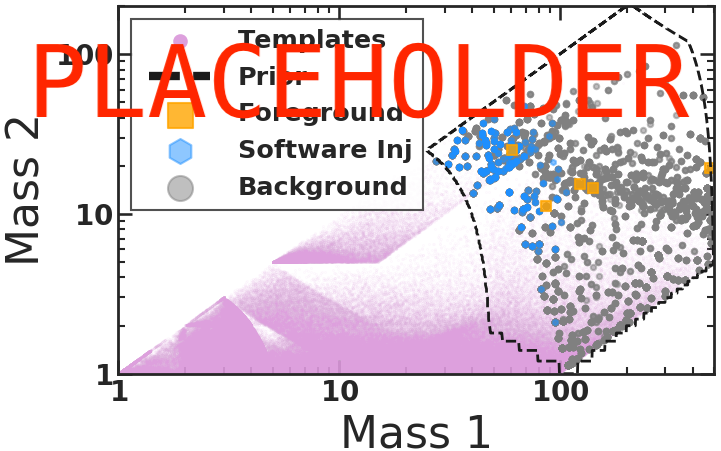
\includegraphics[width=0.75\linewidth]{images/template_bank_masses} 

}
% time for chunk 14
% 1176955218, Apr 23, 2017, 4:00 UTC
% 1178294418, May 08, 2017, 16:00 UTC
\caption[High-mass BCR search space.]{The template bank used by \pycbc to search a section of O2 data from $\text{April 23 - May 8, 2017}$. Our search is constrained to the high-mass parameter space enclosed by the dashed line.}\label{fig:templateBank}
\end{figure}


\subsection{Calculating the BCR for triggers}
To evaluate $Z^S$, $Z^G_i$ and $Z^N_i$ as shown in Eqs.~\ref{eq:zn}-\ref{eq:zg} and calculate the \bcr Eq.~\ref{eq:bcr} for these triggers, we carry out Bayesian inference with \bilby \cite{bilby}, employing \dynesty \cite{dynesty} as our nested sampler. Nested sampling, an algorithm introduced by \cite{skilling_nested_sampling}, provides an estimate of the true Bayesian evidence and is often utilised for parameter estimation within the LIGO collaboration \cite{bilby}.\\ 

The most computationally intensive step during Bayesian inference is the evaluation of the likelihood $\mathcal{L}(d_i|\mu(\vec{\theta}))$. To accelerate our analysis, we use a likelihood that explicitly marginalises over coalescence time, phase at coalescence, and luminosity distance (Eq.~80 from \citet{intro_to_gw_bayes}). While this marginalised likelihood reduces the run time without introducing errors to our evidence evaluation, it does not generates samples for the marginalised parameters. However, these parameter samples can be calculated as a post-processing step \cite{intro_to_gw_bayes}.\\

We set the priors $\pi(\vec{\theta}|\mathcal{H}_S)$ and $\pi(\vec{\theta}|\mathcal{H}_G)$ to be identical. These priors restrict signals with mass parameters in the ranges presented in Table\textasciitilde\ref{tab:parameters}. The spins are aligned over a uniform range for the dimensionless spin magnitude from $\left[0,1\right]$. The luminosity distance prior assigns probability uniformly in comoving volume, with an upper cutoff of $5\ \text{Gpc}$. The remaining priors are the same as the those used for in GWTC-1. \\

The waveform template we utilise is \imrphenomp, a phenomenological waveform template constructed in the frequency domain that models the in-spiral, merger, and ringdown (IMR) of a compact binary coalescence \citep{khan2016frequency}. Although gravitational wave templates such as \seob \cite{seob} created from numerical relativity simulations incorporate more physics such as information on higher-order modes, we still use \imrphenomp as it evaluates faster than numerical relativity models \rs{NOTE: SOEOB is not a NR waveform. It's just tuned to NR}. \\

To generate the PSD \psd \rs{see comment about difference between the psd and the noise variance}, we take 31 neighbouring, off-source, non-overlapping,  $4\ s$  segments of time-series data prior to the data segment $d_i$ being analysed. A Tukey window with a roll off of $0.2\ \text{s}$ is applied to each data segment to suppress spectral leakage after which the segments are fast-Fourier transformed and median-averaged to create a \psd \cite{ligo_psd}. This method, like other \psd estimation methods, adds statistical uncertainties to the \psd \cite{psd_student_t}. To marginalise over the statistical uncertainty we use the median-likelihood presented by \citet{psd_student_t} as a post-processing step and shift our Bayesian Evidence estimations closer to their true astrophysical values. \\ 

Finally, we neglect detector calibration uncertainty and acquire data from from the Gravitational Wave Open Science Center \cite{GWOSC}. The data we use is the publicly accessible O2 strain data from the Hanford and Livingston detectors. To ensure the data is usable we verify that the analysis and PSD data are obtained when the detectors are  in ``Science Mode''. The data requisition and quality checks are conducted using \gwpy \cite{gwpy}. \\

The run-time to calculate a single Bayesian evidence after using \dynesty with $1,000$ live points and $100$ walkers is usually between $0.5-12\ \text{hours}$ (where the run time often depends on the SNR of the data segment). \\

\subsection{Assigning $p_{astro}$ to candidate events}

After the calculating the \bcr for the entire set of high-mass background and simulated triggers, we calculate probability distributions $p_b(\text{BCR})$ and $p_s(\text{BCR})$ for each 2-week time-frame of O2 data. These distributions are used to obtain the ``tuned'' prior-odd $\alpha$ and $\beta$ values that maximise $D_{KL}(p_b|p_s)$ for each time-frame of data.\\

Finally, using the tuned prior odds the \bcr for the candidate events can be calculated. Figure~\ref{fig:bcrCdf} shows the \bcr distributions for the background triggers, simulated triggers and candidate events. The bulk of the background and simulated trigger distributions are separate but have a slight overlap due to some of the simulated signal's being very faint \av{but the BCR should still be able to find the injections and set them to have high BCRs? Could it be that the signals are injected over sketchy-glitch like data? How can I verify this?} \rs{you expect that some genuine signals will be reported as a glitch or noise, e.g., an odds of 1/10 means that you expect that 1 time out of ten a signal is mis classified a noise, and vice versa. You can get a signal at any bayes factor}. This suggests that the \bcr can successfully distinguish signals from noise or glitches. The vertical lines in Figure~\ref{fig:bcrCdf} displays the \bcr for gravitational wave candidate events. On comparing the candidate event \bcr values with the background distribution, we can estimate $p_\text{astro}$ values for the candidate events. 


\begin{figure}[!h]
{\centering 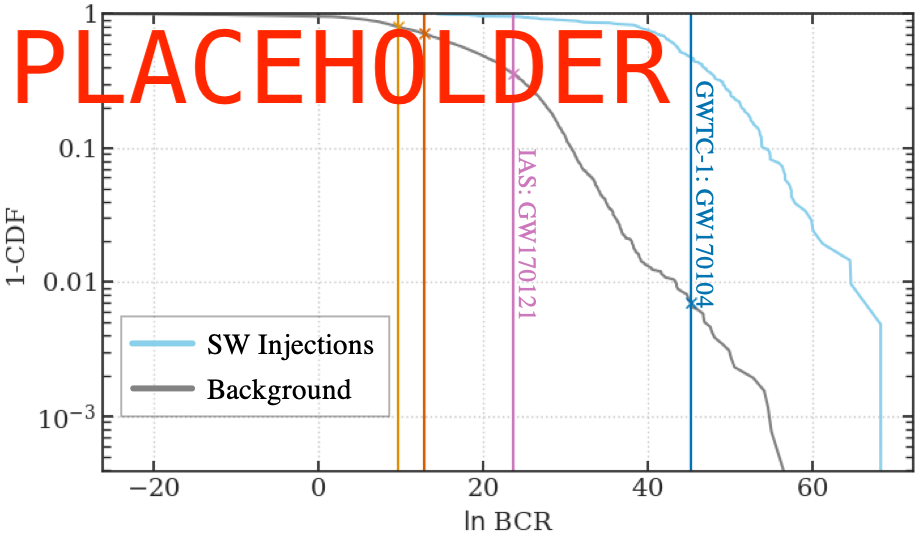
\includegraphics[width=0.75\linewidth]{images/bcr_cdf} }
\caption[BCR distribution example]{Histograms represent the survival function (1-CDF) from our selection of $\sim$ 3,000 background triggers (grey) and 648 simulated signals (blue) triggers obtained from \pycbc's search of data from $\text{April 23 - May 8, 2017}$. Vertical lines mark the ln BCRs of two glitches (orange and yellow), IAS's GW170121 (pink), and GWTC-1's GW170104 (dark blue).}\label{fig:bcrCdf}
\end{figure}






\section{\label{sec:Results}Results}
\av{I should use Pratten et al's table + values here}
In aLIGO's first two observing runs, eleven gravitational wave events were found in the data by the LIGO-Virgo scientific collaboration \citep{abbott2019gwtc}. Since the public release of LIGO's first and second observing run's data, several groups have searched the data for gravitational waves independently of LIGO. One particular research group of interest is a research team at the Institute for Advanced Study (IAS). The group constructed searches to look for the LIGO-confirmed the gravitational wave events detected by the LIGO-Virgo collaboration, and in the process of doing so, claim to have discovered several others events \citep{IAS0, IAS1, IAS2}. Some of these events have total masses $>85$ \msun, which is larger than the average total mass of the LIGO detections. Some of these IAS and LIGO events are displayed in Table\textasciitilde\ref{tab:O2significancesWObcr} with their $p_\text{astro}$ reported by various LIGO and IAS search pipelines.\\

\begin{table}
\caption[\rs{Put BCR first and put a box around it, indicating that this is the new results that people should focus on}$p_\text{astro}$ for various O2 foreground triggers]{\label{tab:O2significancesWObcr}$p_\text{astro}$ from several detection pipelines for a subset of the O2 foreground triggers.}
\centering
\begin{tabular}{lllllll} 
\hline
\textbf{Event} & \textbf{Catalogue} & \textbf{PyCBC} & \textbf{GstLAL} & \textbf{cWB} & \textbf{IAS} & \textbf{BCR} \\ 
\hline
GW170104 & GWTC-1 & 1 & 1 & 1 & 0.99 & 0.99 \\
GW170121 & IAS-1 & NA & NA & NA & 0.99 & 0.65 \\
GWC170402 & IAS-2 & NA & 0.086 & NA & 0.68 & 0.33 \\
GW170403 & IAS-1 & NA & NA & NA & 0.56 & 0.33 \\
IMBHC170423 & IMBH-marginal & NA & 0.95 & 1 & NA & 0.01 \\
GW170425 & IAS-1 & NA & NA & NA & 0.77 & 0.36 \\
GW170502 & Udall et al. & NA & NA & NA & NA & 0.40 \\
GW170729 & GWTC-1 & 0.52 & 0.98 & 0.94 & NA & 0.98
\end{tabular}
\end{table}



From \sout{this} Table\textasciitilde\ref{tab:O2significancesWObcr}, it is evident there is some uncertainty if these events can be considered real gravitational-wave events -- are these events significantly different from the background or not? The various pipelines have different answers. Our \bcr $p_\text{astro}$ shows support that the LIGO-VIRGO events come from an astrophysical source, while the candidate events from the IAS group appear to have a lower probability of originating from an astrophysical source.\\







\section{\label{sec:Conclusion}Conclusion}


\rs{lead with something specific to your work; what did you find/learn? how can it be extended? what does it imply for high mass BBH? How do the reported BCRs on interesting events compare to other bayesian measures of significance/odds? etc...It might be useful to take a look at some of the pycbc search papers for how to summarize results from a search}The detection of high mass black holes $>100$ \msun will shed light on the formation of globular clusters, supermassive black holes and thus galaxy formation \citep{lodato2006supermassive, 2018IMBHreview}. LIGO is theoretically sensitive to the merger of binary black holes with total masses up to 500 M \msun which are expected to occur at a rate of 0-10 yr\(^{-1}\) \cite{mandel2008rates, fregeau2006imbhbRatePrediction}. However, even after \citet{ligo_imbh_search}'s targeted match-filter based search for gravitational waves from high-mass black holes the largest total mass detected so far is approximately 80 \msun \citep{abbott2019gwtc}. A possible explanation for the absence of high mass events may be due to their misclassification as short-duration instrumental noise transients \citep{blipGlitches}. High-mass mergers have very few in-band wave cycles, and hence can easily be mistaken for short-duration instrumental transients. \\

We have developing a targeted search for gravitational waves from high-mass black hole systems. This targeted search utilises Bayesian inference and provides a ranking statistic that contains a lot of physical information about the high-mass systems. We have applied this technique on all the high-mass triggers identified by \pycbc during LIGO's second observing run to investigate the possibility of discovering new gravitational-wave signals from high mass black hole binaries. Although we were unable to uncover new gravitational waves events, we were able to report high $p_{astro}$ for events already detected by LIGO, and low $p_{astro}$ for some events identified by external pipelines. 
%%%%%%---SECTIONS-END---%%%%%%%%%%%%

%%%%%%---ACKNOWLEDGEMENTS---%%%%%%%%%%%%
\begin{acknowledgments}

This research has made use of data, software and/or web tools obtained from the Gravitational Wave Open Science Center (https://www.gw-openscience.org), a service of LIGO Laboratory, the LIGO Scientific Collaboration and the Virgo Collaboration. LIGO is funded by the U.S. National Science Foundation. Virgo is funded by the French Centre National de Recherche Scientifique (CNRS), the Italian Istituto Nazionale della Fisica Nucleare (INFN) and the Dutch Nikhef, with contributions by Polish and Hungarian institutes.

\end{acknowledgments}
%%%%%%%%%%%%%%%%%%%%%%%%



\bibliography{high_mass_bib}% Produces the bibliography via BibTeX.

\end{document}
%
% ****** End of file apssamp.tex ******
